\section{Catrobat Android Apps}
\label{section-catrobat-case-study}

\setminted{fontsize=\small,baselinestretch=1}

\subsection*{Evidence}
  \begin{minted}[
    gobble=4,
    frame=single,
    fontsize=\tiny,
    breaklines=true
  ]{yaml}
    evidence available :
      vitals-scraper : ~/sandbox/vitals-scraper-logs/android-stability-analysis/data/from-android-vitals
      google-play-console-reports : ~/Dropbox/Google Play Console Reports/reports/catrobat/pocketcode/crashes
      various-materials : in Dropbox
      co-written-paper : WAMA 2019
    evidence-needed : 
      Releases and their release dates.
      Latest status of the tickets raised at the hackathon.
      Current stability metrics for the 2 apps.
  \end{minted}

%%%%%
% Stuff on minted
% https://tex.stackexchange.com/questions/35546/minted-setstretch-and-font-size
% https://tex.stackexchange.com/questions/484788/how-to-change-overall-font-size-of-minted
% https://tex.stackexchange.com/questions/399340/change-font-size-in-minted
% https://tex.stackexchange.com/questions/531738/minted-environment-not-working-in-overleaf
% Revisit the following if I include minted more often https://tex.stackexchange.com/questions/103141/set-global-options-for-inputminted

\subsection{Abstract}
We ran a 1-day hackathon with six of the core development team for the Pocket Code Android app where we identified the top ten crashes and top ten ANRs for the app using reports provided in Android Vitals. These were recorded in the project's JIRA system; the crash reports were correlated with Fabric Crashlytics also used in the Pocekt Code app. The team worked on a subset of these 20 issues during the hackathon and in the following weeks. The crash rate was halved within 2 releases of the app and six weeks of the hackathon. 

The improvement was particularly impressive as the team's clean coding practices and their sophisticated `best practices' had not managed to effect a similar improvement in the previous months. Further scope for improvement is likely. However, the improvements petered out after the the owner for runtime stability left the team shortly after these two releases were deployed. New stability issues have emerged in more recent releases, indicating a tendency to entropy in codebases and their products unless runtime failures are actively monitored and addressed.

Changes enforced by Google led to the migration from Fabric Crashlytics to Firebase Crashlytics for reporting purposes. The team discovered personal information was being collected and reported by Google \textit{despite the Crashlytics SDK remaining unchanged and intended only to report on crashes and errors}. The project leader chose to stop actively using Crashlytics in the project as a result in order to protect the privacy of the end users.

% Applying advice from https://nssmic.ieee.org/2019/wp-content/uploads/sites/2/2019/02/Abstract_Style_Guide.pdf
% See also https://conferences.ieeeauthorcenter.ieee.org/write-your-paper/structure-your-paper/ 

\subsection{Introduction to the Catrobat Case Study}
% Joe's notes this is not compelling and doesn't compare with the other case studies.
% Why Catrobat, what did I gain, similarities and contrasts, why include in the PhD.
% Existing best practices, assiduously applied didn't reduce the crash rate, my approach did! :)
% Needs to be applied on a long term basis.

This case study includes an extremely and unusually well researched and properly developed app and codebase where many of the perceived good practices were and are assiduously applied on an ongoing basis. The codebase is far more complex than the Kiwix Android apps and the app is significantly richer in terms of the features and functionality.

This case-study includes some in-app analytics, in the form of a crash reporting tool called Crashlytics. This additional source of analytics identified additional concerns with analytics tools as the two sources of analytics (Google Play Console and Crashlytics) had significant differences in their calculations and reports. It illustrates the efficacy of investigating crashes reported by the analytics where relatively minor effort was needed to identify and fix causes of poor reliability.

Furthermore, the project team chose to invest their energies into supporting a testing workshop in Poland and to introducing application-level in-app analytics to both their Android and iOS PocketCode apps. Their actions indicate the project team recognise the benefits of applying and incorporating analytics into their software development and quality improvement practices.

\subsection{Potted History of the Project}
\begin{enumerate}
    \item Rationale:
    \item Involvement of under-grads and post-grads. Master's theses (ask for stats).
    \item External contributors: translations, rich community contributions of PocketCode apps, ...
    \item Catrobat foundation, and funded work.
    \item Software Development, testing, maintenance,...
\end{enumerate}
Rationale,
Involvement of under-grads and post-grads. Master's theses (ask for stats)
Catrobat foundation, and funded work.

\subsubsection{Catrobat Software Engineering Practices}
Approach to development, testing, deployment, production monitoring, ...

The project uses Jenkins to run continuous builds for PocketCode and other related projects \url{https://jenkins.catrob.at/job/Catroid/}. Most of the builds are for the Develop code branch \url{https://jenkins.catrob.at/job/Catroid/job/develop/}.

At the start of the case study the crash rate of the Pocket Code app remained stubbornly high despite the extensive use of code quality tools and practices, automated testing, continuous builds and so on. In the product view of quality, ~\citep{kitchenham1996_software_quality_elusive_target}, observed that the approach of taking a product view of quality~\emph{``is frequently adoptd by software-metrics advocates, who assume that measuring and controlling internal product properties (internal quality indicators) will result in improved external product behavior (quality in use)."}~\footnote{US English spelling was used in the original article so used here in the quotation.} Back when the article was published, in 1996, the authors stated \emph{``more research was needed to determine which aspects of internal quality affect the product's use."}

\subsection{Method}
Discussions, co-organised a hackathon in Graz, Austria at the project's parent university, planned for 24 hours from 9am 16th November 2019. 

Hackathon focus: to improve code quality based on failures and issues reported in Android Vitals (cross-referenced with those reported in Fabric Crashlytics).

\subsection{The Project's Working Practices}
Specific roles, who can do what.
Issues need to be reported in JIRA in order for any code to be considered

\subsection{Introduce the Analytics Tools}
\begin{enumerate}
    \item Types of crashes: Soft crashes (mapping terminology between Fabric Crashlytics and Android Vitals).
\end{enumerate}

\subsection{Summary of the Hackathon}
The visit (including the presentation at the Graz University of Technology on Friday morning and to Dynatrace\footnote{\url{https://www.dynatrace.com}} on Friday afternoon) helped reinforce the value of creating and using the Vitals-Scraper software to preserve history. 

There was a peak of eight participants from the Catrobat team during the hackathon. This included two people %(including Wolfgang and Matthias)
in non-coding capacities. Approximate time spent. Twenty-two (22) issues were raised during the day (tagged: hackathon-2019)\footnote{\url{https://jira.catrob.at/browse/CATROID-426?jql=labels\%20\%3D\%20hackathon-2019}}. Most of these were created in the morning, one for each of the top crashes and ANRs as recorded and ranked in Android Vitals. 

\subsection{Immediate Results}
We can group the issues using as follows (already fixed, addressed during the hackathon, pending, rejected).

\subsubsection{Already fixed} JIRA issue 405\footnote{\url{https://jira.catrob.at/browse/CATROID-405}} was the \#1 issue with over 2000 crashes reported in the 30 days preceding the hackathon (and over 3200 in the lifetime of the app). However, it had already been addressed in JIRA issue 379\footnote{"media download progress dialog crashers" \url{https://jira.catrob.at/browse/CATROID-379}} and incorporated in to the most recent release \footnote{Release:
0.9.65 Nov 13, 6:01 PM: Full rollout.} as part of a major effort to improve the code quality around the embedded WebView component.

Early indications are that the fixes related to the WebView have made a material improvement in the crash-rate for PocketCode 2.45\% vs. 3.9.3\% on Monday \nth{18} November 2019; details are in Table \ref{tab:androidvitals_rollout_of_0_9_65}. Therefore, in terms of assessing any improvement that results from the work of the hackathon the baseline is 2.45\%.

% TODO perhaps move these to a Glossary section?
% Number of sessions tool-tip: Approximate number of recorded sessions
% Crash-free sessions tool-tip: Percentage of daily sessions during which your users did not experience any crashes. A daily session refers to a day during which your app was used.
% Impacted sessions tool-tip: Percentage of daily sessions during which your users experienced at least one crash. A daily session refers to a day during which your app was used.
\begin{table}[htbp!]
    \centering
    \footnotesize
    \begin{tabular}{r|r|r|r}
        App version &Impacted sessions &Crash-free sessions &Number of sessions  \\
        \hline
        69 (0.9.65) &2.45\% &	97.55\% 	&~800 \\
        Production &&& \\
        \hline
        66 (0.9.64) &3.93\% &96.07\% 	&~3K
    \end{tabular}
    \caption{AndroidVitals: Improvement in crash-rate post WebView improvements}
    \label{tab:androidvitals_rollout_of_0_9_65}
\end{table}

The change was to remove a progress dialog for media downloads. The development team was not able to reproduce the crash according to the JIRA ticket or the code review in the pull request \#3362\footnote{\url{https://github.com/Catrobat/Catroid/pull/3362/files}}. And yet the fix seems to have had the desired effect in terms of the crash rate. The effect on the UX is not known.

\subsubsection{Addressed During the Hackathon}
Some of the issues were determined to be 'soft errors' that were leaking to Android Vitals even though the app handled / recovered from them. These were addressed through the work recorded in  \href{https://jira.catrob.at/browse/CATROID-426}{CATROBAT-426}. Table \ref{tab:hackathon_2019_jira_addressed} provides a brief summary of all the issues addressed in the hackathon.


\href{https://jira.catrob.at/browse/CATROID-418}{CATROID-418 - Crash in PlaySoundAndWaitBrick.addActionToSequence} The author paired with one of the developers on this issue. It is believed to be a bug that can only occur at runtime when the user has deleted the sound file that is being used by the \texttt{PlaySoundAndWaitBrick} which raised an \texttt{IllegalArgumentException} as it cannot determine the path from the Java Object that represented the sound file for this PocketCode visual programming element. We were able to reproduce the error on a local device and implement a fix. The developer thought a similar behaviour might be the cause of the exception reported in issue \href{https://jira.catrob.at/browse/CATROID-419}{419}, this has yet to be investigated.

\begin{table}[htbp!]
    \footnotesize
    \centering
    \begin{tabular}{rll}
        JIRA Ticket &Category &Remarks \\
        \hline
        \href{https://jira.catrob.at/browse/CATROID-407}{CATROBAT-407} &NullPointerException &Soft error already handled by app. \\
        \href{https://jira.catrob.at/browse/CATROID-409}{CATROID-409} &NullPointerException &Crash in showLegoSensorConfigInfo
        \\
        \href{https://jira.catrob.at/browse/CATROID-418}{CATROID-418} &IllegalArgumentException &Crash in \\&&  PlaySoundAndWaitBrick.addActionToSequence \\
        %SHOULD_DO fix Temporary hack to wrap above text.

    \end{tabular}
    \caption{Hackathon bugs addressed during hackathon.}
    \label{tab:hackathon_2019_jira_addressed}
\end{table}

\subsubsection{Pending} 
Table \ref{tab:hackathon_2019_jira_issues_pool} summarises the issues that were raised and were not actioned during the hackathon.

Of these, \href{CATROID-410}{https://jira.catrob.at/browse/CATROID-410} and \href{https://jira.catrob.at/browse/CATROID-412}{CATROID-412}seem, as issue \href{CATROID-405}{https://jira.catrob.at/browse/CATROID-405} was, to have been fixed in the recent release 0.9.65 (69). Android Vitals shows these crashes last occurred in the previous release of 0.9.64 (66).

Similarly, issues \href{https://jira.catrob.at/browse/CATROID-413}{CATROID-413 - Crash in saveScreenshot} has not yet been reported for the current release: 0.9.65 (69).

\href{CATROID-411}{https://jira.catrob.at/browse/CATROID-411} is for an ANR (where the app freezes) when taking a screenshot. This occurs in both the previous and current releases and is currently being investigated by one of the development team.

\href{https://jira.catrob.at/browse/CATROID-413}{CATROID-413 - Crash in LineTool.draw} seems to be a long-running issue, found in releases (65), (66), and the current release (69).

\href{https://jira.catrob.at/browse/CATROID-415}{CATROID-415 - Crash in onBackPressed} is another long-running release however it is happening much more often - twenty-eight times by Monday \nth{18} November 2019 in the current release (69), versus once in release 63 (on \nth{23} October 2019. Of the crashes in (69) happened on the same day as the hackathon - perhaps the participants were triggering albeit they might not be aware of it? If they weren't aware, this might be another instance where the issue is a 'soft-error' which is handled by the app and therefore suitable for similar treatment to that proposed in \href{https://jira.catrob.at/browse/CATROID-426}{CATROID-426}?

\href{https://jira.catrob.at/browse/CATROID-416}{CATROID-416 - Crash in VisualPlacementActivity} from Android Vitals, this crash has only been reported in the current release 0.9.65 (69). It affected a range of devices and occurred on at least 2 Android versions.

\href{https://jira.catrob.at/browse/CATROID-417}{CATROID-417 - Crash in MainMenu onCreate} may be newly introduced in 0.9.65 (69). This has only been reported for a single user who experienced it 4 times. The exception is a \texttt{java.lang.ClassCastException} perhaps it's triggered by a particular PocketCode script or method call?

\href{https://jira.catrob.at/browse/CATROID-420}{CATROID-420 - Crash in resolveFileName} This was addressed two days after the hackathon and merged into the next release 0.9.66 (70). The crash was newly reported in 0.9.65 (69) and happened twice, once on an Huawei Y9 and once on an Honor 7X.

\href{https://jira.catrob.at/browse/CATROID-421}{CATROID-421 - ANR in MainMenuActivity} This ANR was reported in both 0.9.64 (66) and 0.9.65 (69) and has been reported on Android 7.0 and 7.1 on 3 distinct device models with all bar one on Xiaomi devices, the remaining crash is on a Lenovo VIBE K6 Note (K53a48), with Android 7.0.

\href{https://jira.catrob.at/browse/CATROID-423}{CATROID-423 - ANR in ProjectActivity} This ANR has also occurred in the most recent release: 0.9.66 (70). It's been reported 7 times on 4 device models in the last 30 days and on both Android 7.0 and 7.1

From the trace, perhaps it's related to taking a screenshot? Also, the queue delay can be over 18 seconds - far longer than anyone would like:

\texttt{\footnotesize{"Input dispatching timed out \\(org.catrobat.catroid/org.catrobat.catroid.ui.ProjectActivity, \\Waiting to send non-key event because the touched window has not finished processing certain input events that were delivered to it over 500.0ms ago. Wait queue length: 28. Wait queue head age: 18726.7ms.)"}}

\href{https://jira.catrob.at/browse/CATROID-424}{CATROID-424 - ANR in SpriteActivity} This ANR is also reported in newer 0.9.66 (70) and older releases, see \ref{tab:catroid_424}:

\begin{table}[htbp!]
    \centering
    \begin{tabular}{r|r|r}
Release	&Instances	&Percent \\
\hline
66	&12	&63.2\% \\
69	&6	&31.6\% \\
70	&1	&5.3\% \\
    \end{tabular}
    \caption{By app version for CATROID-424 issue}
    \label{tab:catroid_424}
\end{table}

The error summary is:

\texttt{\footnotesize{
Input dispatching timed out (AppWindowToken{c8e9f token=Token{b3ee03e ActivityRecord{4ed08f9 u0 org.catrobat.catroid/.ui.SpriteActivity t12205}}}, Waiting because no window has focus but there is a focused application that may eventually add a window when it finishes starting up.)}}

\href{https://jira.catrob.at/browse/CATROID-425}{CATROID-425 - tgkill crashes} There are various crash clusters for \texttt{tgkill}, 19 in 60 days to \nth{1} December 2019 across all versions of the app and Android versions. These have not been investigated yet. The ticket includes references to various guides to help investigate the causes.

\begin{table}[htbp!]
    \centering
    \footnotesize
    \begin{tabular}{r|l|l}
        JIRA Ticket &Category &Remarks \\
        \hline
        \href{https://jira.catrob.at/browse/CATROID-406}{CATROBAT-406} &NullPointerException &...BrickBaseType.getDragAndDropTargetList. \\
        \href{https://jira.catrob.at/browse/CATROID-408}{CATROID-408} &NullPointerException &Crash in Save Project. \\
        \href{https://jira.catrob.at/browse/CATROID-410}{CATROID-410} &NullPointerException &Crash in saveLegoNXTSettingsToProject \\
        \href{https://jira.catrob.at/browse/CATROID-411}{CATROID-411} &ANR &\texttt{StageListener.takeScreenshot} \\
        \href{https://jira.catrob.at/browse/CATROID-412}{CATROID-412} &NullPointerException &Crash in SetBackgroundEventId.hashCode \\
        \href{https://jira.catrob.at/browse/CATROID-413}{CATROID-413} &NullPointerException &Crash in saveScreenshot \\
        \href{https://jira.catrob.at/browse/CATROID-414}{CATROID-414} &NullPointerException  &Crash in LineTool.draw \\
        \href{https://jira.catrob.at/browse/CATROID-416}{CATROID-416} &NullPointerException &Crash in VisualPlacementActivity \\
        \href{https://jira.catrob.at/browse/CATROID-417}{CATROID-417} &ClassCastException &Crash in MainMenu onCreate \\
        \href{https://jira.catrob.at/browse/CATROID-420}{CATROID-420} &SecurityException &Crash in resolveFileName \\
        \href{https://jira.catrob.at/browse/CATROID-421}{CATROID-421} &ANR &MainMenuActivity \\
        \href{https://jira.catrob.at/browse/CATROID-423}{CATROID-423} &ANR &ProjectActivity \\
        \href{https://jira.catrob.at/browse/CATROID-424}{CATROID-424} & ANR &SpriteActivity \\
        \href{https://jira.catrob.at/browse/CATROID-425}{CATROID-425} &tgkill &Various crash clusters \\
    \end{tabular}
    \caption{Hackathon bugs in the "Issues Pool"}
    \label{tab:hackathon_2019_jira_issues_pool}
\end{table}

\subsubsection{Rejected}
\href{https://jira.catrob.at/browse/CATROID-422}{CATROID-422 - Crash at org.catrobat.catroid.ui.ProjectActivity.showLegoSensorConfigInfo } \texttt{(ProjectActivity.java:396)} %TODO work out why I needed to split the above to avoid a latex compile error.
This was rejected by one of the developers as they wanted to suppress the crash (which is considered one the app recovers from) through \href{https://jira.catrob.at/browse/CATROID-426}{CATROID-426}. Interestingly the 'fix' did not stop this crash from being reported in 0.9.66 (70).

\subsubsection{Permission Denials}
One of the Android Vitals "qualities" pertains to how often users deny permissions requested by an app. A low percentage (ideally zero) is their target recommendation. As Table \ref{tab:pocketcode_permission_denials} shows, PocketCode has a significant percentage of denials, 4.74\% as of \nth{18} November 2019. In discussion with the project lead % Commented out for review purposes:  , Prof. Wolfgang Slany, 
during the hackathon, this is a known consideration. The project team aims to improve the behaviour (\emph{i.e.} the design and implementation). The app currently asks users early on for permission to check the memory card in order to find PocketCode projects. As the permission dialog asks about access to read photos and videos, etc.\todo{Add screenshot and correct wording} it does not seem relevant to some users and they say no. As others have determined\todo{add references to design and timing of when to ask users things}  when and how an app asks a user has affects the outcomes.


% The following was copy-pasted from Android Vitals on 18th Nov 2019 for the PocketCode app.
% Metric 	Last 30 days 	Previous 30 days vs. peers’ median The difference between you and the peers’ median
% Permission denials Percentage of daily permission sessions during which users denied permissions. A daily permission session refers to a day during which your app requested at least 1 permission from its user. If a user makes multiple decisions for the same permission, only the final decision at the end of a day is recorded. Transparently explaining the reasons for permission requests can help reduce permission denials. 	4.74% 	4.39% 	-

% https://play.google.com/apps/publish/?account=8841632091579025670#AppHealthDetailsPlace:p=org.catrobat.catroid&appid=4975762901432177859&aho=APP_HEALTH_OVERVIEW&ahdt=PERMISSION_DENIAL&ts=THIRTY_DAYS&ahbt=_APPLICATION


  \bxtable[htbp!]{{AndroidVitals: PocketCode: "Permission Denials"}}
  {
  \begin{minipage}{16cm}
  %\begin{center}
    \begin{tabular}{lrrr}
        Metric 	&Last 30 days\footnote{As of \nth{18} Nov 2019} 	&Previous 30 days &vs. peers’ median  \\
        Permission denials\footnote{Percentage of daily permission sessions during which users denied permissions.\\ A \emph{daily permission session} refers to a day during which your app requested at least 1 permission from its user. If a user makes multiple decisions for the same permission, only the final decision at the end of a day is recorded. Transparently explaining the reasons for permission requests can help reduce permission denials~\citep{androiddevelopers2020_permission_denials}} & 4.74\% 	&4.39\% 	&- \\
   
   \label{tab:pocketcode_permission_denials}
    \end{tabular}
     % \end{center}
  \end{minipage}
  \centering
}

% Thanks to https://tex.stackexchange.com/questions/10181/using-footnote-in-a-figures-caption for the local footnotes.
% This also helped me find a viable approach: https://tex.stackexchange.com/questions/109467/footnote-in-tabular-environment
% This also looks good as an alternative: https://texblog.org/2012/02/03/using-footnote-in-a-table/
% Ditto the following threeparttable example https://blog.modelworks.ch/tables-with-footnotes-in-latex/

% And yet more reading in an attempt to quiesce nag messages (I've yet to succeed)
% https://latex.org/forum/viewtopic.php?t=31733
% https://tex.stackexchange.com/questions/237549/center-environment-nag-warning-for-floats-in-beamer

% Tables ain't trivial in latex. Finally the following article clearly explains how to use captionof minipage and tabular
% https://tex.stackexchange.com/questions/15282/tabular-title-above-and-caption-below
% and https://tex.stackexchange.com/questions/2275/keeping-tables-figures-close-to-where-they-are-mentioned

\subsubsection{1 Week on}
Release 0.9.65 is now the dominant release, with ~4000 sessions between \nth{17} and \nth{23} November, compared to ~600 sessions for the previous release of the app (0.9.64). The overall reported crash rate reduced to 2.10\% for \nth{18} to \nth{23} November, compared to the previous 7 days crash rate of 3.62\%. \textbf{Note these are for releases that predates the hackathon.}

During a call with Professor Slany on \nth{25} November, he mentioned they had planned to release a new version of the app on Friday to address the loss of Fabric Crashlytics data and several improvement related to the hackathon; however their Jenkins build was coincidentally broken that day \url{https://jenkins.catrob.at/job/Catroid/job/develop/1098/} where the build failed to complete for over 54 hours. The cause was being investigated. According to logs on Jenkins it may be related to Docker not being available \texttt{Cannot connect to the Docker daemon at unix:///var/run/docker.sock. Is the docker daemon running?} \footnote{\url{https://jenkins.catrob.at/view/Catroid/job/Catroid/job/develop/1102/execution/node/27/log/}}

\subsubsection{2 weeks on}
\nth{1} December 2019.

A new release of the app was launched on November \nth{26} after several days of problems with the Jenkins CI pipelines which delayed this release by about 4 to 5 days.

The new release 0.9.66 (70) seems to have made a slight improvement to the overall crash rate which is currently 1.95\% after 3 days of data in Android Vitals, the previous release has a crash rate of 2.56\% for the last 7 days (to \nth{29} November. It is premature to determine the overall effect of the crash rate for this app as it's still being rolled-out (which typically takes over a week to reach the majority of the user-base e.g. on \nth{2} December (4 days after the release started rolling out) Android Vitals reports 20K install events).

The ANR rate is also showing encouraging signs, for the last 7 days (actually it seems to be only for 6 days, from \nth{24} to \nth{29} November 2019 as reported on \nth{1} December 2019) in Table~\ref{tab:ANR_rate_24_to_29_Nov_2019}.

\begin{table}[htbp!]
    \centering
    \footnotesize
    \begin{tabular}{r|r|r|r}
      App version  &Impacted sessions &ANR-free sessions &No. sessions \\
      \hline
      70 (0.9.66) Production &0.30\% &99.70\%	&~700 \\
      69 (0.9.65)            &0.46\% &99.54\%	&~3K  \\
    \end{tabular}
    \caption{PocketCode: ANR rate for Last 7 days}
    \label{tab:ANR_rate_24_to_29_Nov_2019}
\end{table}

\subsection{Progress in cumulative releases}

% MUST_DO add screenshots and summaries of the progress made with subsequent releases of Pocket Code for Android.

\begin{table}[htbp!]
    \centering
    \footnotesize
    \tabcolsep=0.06cm
    \begin{tabular}{r|r|r|r|r}
    \small
        App version &Impacted sessions &Crash-free sessions &Number of sessions &Period \\
        \hline
        72 (0.9.68) &1.26\% &   98.74\%     &~9K  &11-Jan-2020 to 08-Feb-2020 \\
        71 (0.9.67) &1.25\% &   98.17\%     &~14K &11-Jan-2020 to 08-Feb-2020 \\
        70 (0.9.66) &1.65\% &   98.35\%     &~5K  &04-Jan-2020 to 01-Feb-2020 \\
        69 (0.9.65) &2.05\% &	97.95\% 	&~2K  &22-Oct-2019 to 19-Nov-2019 \\
        \hline
        66 (0.9.64) &3.61\% &   96.39\% 	&~16K &22-Oct-2019 to 19-Nov-2019 \\
    \end{tabular}
    \caption{AndroidVitals: Improvement in crash-rate post Hackathon}
    \label{tab:androidvitals_crashrate_post_hackathon}
\end{table}

Some notes on Table~\ref{tab:androidvitals_crashrate_post_hackathon}:
\begin{enumerate}
    \item The data was reported for thirty day periods, one of three durations available in the user interface. All figures were calculated and provided by Google's Android Vitals analytics.
    \item The reports exclude small aggregate counts that fail to meet Google's reporting thresholds.
    \item The percentages fluctuate depending on where releases are in their maturity (their production lifecycle). Therefore these values are spot figures calculated that day and indicative rather than necessarily being suitable for calculating ratios for different periods.
    \item These reports appear to be regenerated once a day, roughly 24 hours apart.
    \item It is unclear whether the underlying data is filtered to limit it to apps only installed by end users of production releases from Google Play.
\end{enumerate}


\subsection{Findings and Results}

Android Vitals `Bad Behavior' alerts colour coded and intended to help developers quickly notice and respond to high error rates, as illustrated in Figure~\ref{fig:android-vitals-pocketcode-alerts-23-jan-2020}. %Evidence AppHealthOverviewPlace_8841632091579025670_org.catrobat.catroid_1579796386172.png

\begin{figure}
    \centering
    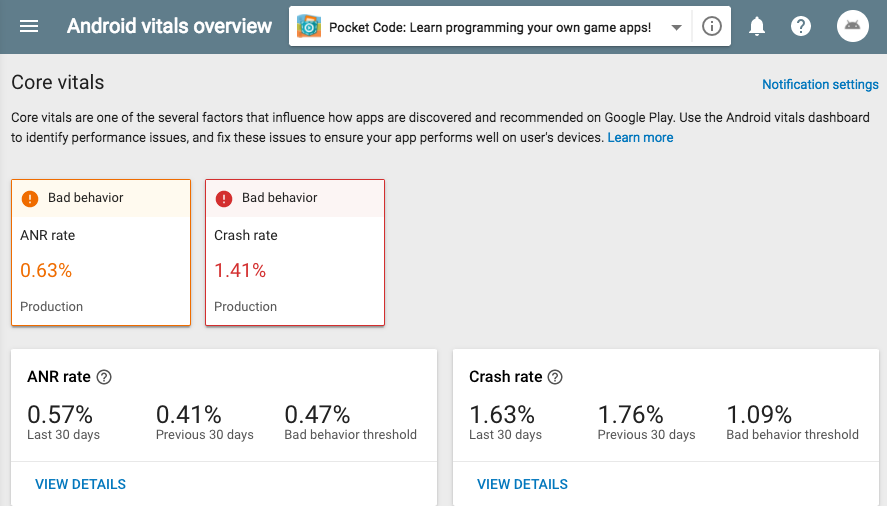
\includegraphics[width=12cm]{images/google-play-console/android-vitals-pocketcode-alerts-23-jan-2020.png}
    \caption{Android Vitals overview, bad behaviours (Pocket Code example)}
    \label{fig:android-vitals-pocketcode-alerts-23-jan-2020}
\end{figure}

No plots for either Pocket Code or Pocket Paint for the ANRs and for the crashes on \nth{10} February 2020, as illustrated in Figure~\ref{fig:android-vitals-pocketcode-broken-graph-10-feb-2020}. 
%Evidence AppHealthDetailsPlace_8841632091579025670_org.catrobat.paintroid_1581848687528.png and AppHealthDetailsPlace_8841632091579025670_org.catrobat.catroid_1581848687528.png and AppDashboardPlace_8841632091579025670_org.catrobat.paintroid_1581848687528  

\begin{figure}
    \centering
    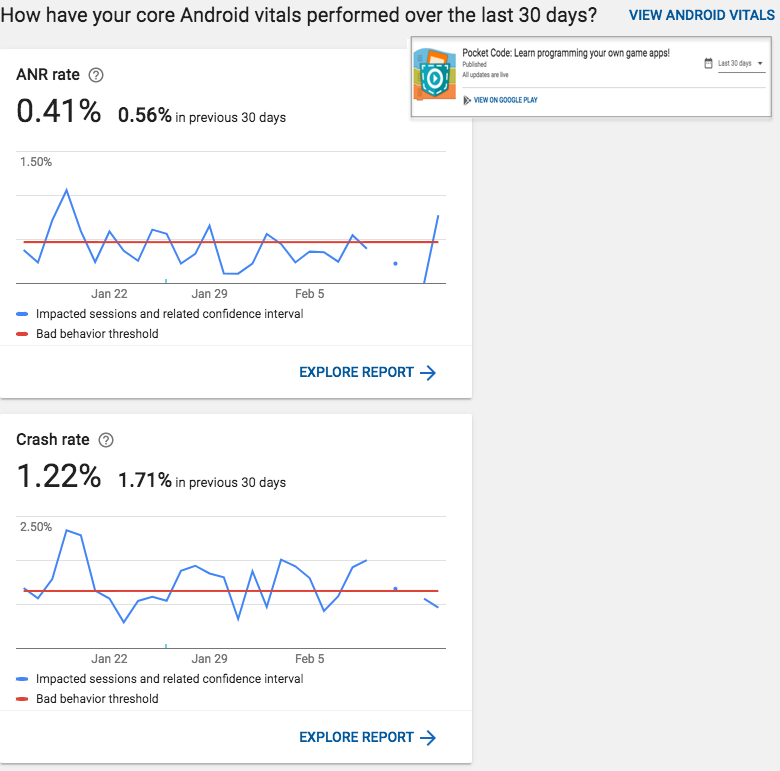
\includegraphics[width=10cm]{images/google-play-console/android-vitals-pocketcode-broken-graph-10-feb-2020.png}
    \caption{Android Vitals graph data missing for~\nth{10} Feb 2020 (Pocket Code example)}
    \label{fig:android-vitals-pocketcode-broken-graph-10-feb-2020}
\end{figure}
Illogical results for installed userbase. %Evidence various graphs.

\subsection{Discussion}
Effects of being measured is a well-known in work, business, etc. One of the effects here was that 'soft-crashes' were reaching Android Vitals and therefore significantly and adversely affecting the crash rate (see \cite{CATDROID-426-JIRA}).

\subsubsection{Validity considerations}
\begin{itemize}
    \item Inconsistencies in the practices
    \item Inconsistencies in the tools
\end{itemize}

\subsubsection{Peer Groups}
The Pocket Code Android app had a significantly higher crash-rate compared to its peer group, as Figure \ref{fig:pocketcode_peer_crash_rate_18_nov_2019} shows in section \href{android-vitals-peer-groups}{\emph{\nameref{android-vitals-peer-groups}}} shows. While this may be undesirable, the Pocket Code app had incredible richness and complexity compared to the perceived peer apps, for instance it includes support for generating native Android apps, an app store, generation of rich, graphical games, as examples of some of the rich capabilities on offer.


\subsubsection{Slower growth of user-base}
PocketCode is an app developed to serve several challenges simultaneously, including research aspects such as the effects of various software development engineering practices, while also being intended to be open, in terms of informing the end-user of the purposes of the app, yet also being easy, fun and educational for children to use in terms of exploring how to write and publish software. These various concurrent challenges led to the users being presented with a long page of legal text (reformatted slightly from the original \href{https://github.com/Catrobat/Catroid/blob/develop/catroid/src/main/res/values/strings.xml}{\textbf{\texttt{Privacy policy on GitHub}}} and reproduced below in Listing~\ref{pocketcode-privacypolicy}). New users are expected to read and agree to before they are allowed to use the app further. Imagine having to scroll through all the text on a small screen \emph{before seeing what the app can do!} The thesis continues after the listing...

% COULD_DO there's lots of scope to tidy up this listing at some point.

\definecolor{dkgreen}{rgb}{0,0.6,0}
\definecolor{gray}{rgb}{0.5,0.5,0.5}
\definecolor{mauve}{rgb}{0.58,0,0.82}

\lstset{frame=tb,
  language=Cobol,
  aboveskip=3mm,
  belowskip=3mm,
  showstringspaces=false,
  columns=flexible,
  basicstyle={\tiny\ttfamily},
  numbers=left,
  numberstyle=\tiny\color{gray},
  %keywordstyle=\color{blue},
  commentstyle=\color{dkgreen},
  %stringstyle=\color{mauve},
  breaklines=true,
  breakatwhitespace=true,
  tabsize=2
}
\begin{multicols}{3}
% \lstinputlisting[{language=[LaTeX]TeX},breaklines=true]{\jobname.tex}

\begin{lstlisting}[caption={Privacy Policy for Pocket Code},captionpos=b,label={pocketcode-privacypolicy}]
Welcome!
Before you can start coding, please read and accept our Privacy Policy to use the app:
To offer you all the benefits of our services and the associated account, it is necessary to collect certain data from you.
* To maintain and improve our services (apps and websites) and to do scientific research on ICT and STEM/STEAM education, we use Google Analytics, Crashlytics, and Firebase, all by Google LLC (USA), as well as Dynatrace by Dynatrace LLC (USA) to get metadata about the usage of our services, e.g., crash information, timestamps, visited pages/screens, usage of our apps and services, used operating system, and information about the network provider. This analysis and the collected data is not linked to your profile and does not contain any personal information (last bits of the IP address get anonymized). However, the collected data will get transferred to the service-provider (Google LLC, USA and Dynatrace LLC, USA). 
Data processing is based on agreements with Google LLC and Dynatrace LLC. 
This relationship to the service provider conforms to the European Union\'s General Data Protection Regulation (EU GDPR) and EU-USA \"Privacy Shield\" agreement.
* To create and use an account in our systems, and to inform you about necessary changes about your account per e-mail, e.g., updates or violations of our Terms of Use and Service, our community rules, or our policies, we will store your username and, if provided by you, your e-mail address. If you have connected your account via your Google or Facebook account, we additionally store an identification key connected to your account on these services. We will not use this data for any other (e.g., marketing) purposes, unless you explicitly allowed us to do so.
* On a voluntary basis, you can give us your country of residence through your account page on the sharing site. This will get displayed on your public profile and only be used for statistical and research purposes by us. It can be removed at any time in your profile settings.
* You can withdraw the usage of the personal data belonging to your account at any time by deleting your account through your profile page on https://share.catrob.at. After deleting your account you will still be able to use the provided services, but not to collaborate, e.g., through uploading programs, commenting, or liking. Also, all provided content linked to your account, e.g., uploaded programs, comments, etc., will be deleted.
* To avoid misuse of our services, e.g., through user contributed uploads or comments for illegal purposes, all user generated public data (uploads, comments) will be stored internally in a database, together with a timestamp and the used internet address. This data will not be used by or forwarded to any institutions, unless sufficiently illegal actions are reasonably suspected and officially entitled legal institutions request it based on applicable law. Each case will be thoroughly checked on an individual basis by us first.
* You can voluntarily subscribe to the Catrobat Newsletter, on https://catrob.at/newsletter provided by us through the MailChimp service (The Rocket Science Group LLC d/b/a MailChimp, USA). You will then receive updates on the Catrobat project and its services to your provided e-mail address. You can withdraw the newsletter at any time by using the \"unsubscribe\" link in the footer of every newsletter. This newsletter is provided by MailChimp with whom we do have a data-processing agreement and who committed to the EU General Data Protection Regulation and EU-USA \"Privacy Shield\". For further details on MailChimp please also look up MailChimp\'s Privacy Policy and Terms of Use.
* All Services are provided by the free open source Catrobat project under the umbrella of the International Catrobat Association - Verein zur Foerderung freier Software, a non-profit NGO incorporated in Graz, Austria (European Union). Our policies pay respect to EU and Austrian data protection law (GDPR). To get in touch with us, please send an e-mail to contact@catrobat.org or mail us to Catrobat,
    c/o
    Institute of Software Technology,
    Graz University of Technology,
    Inffeldgasse 16b,
    A-8010 Graz, Austria
    (European Union).
In case you are below the age of 14, this policy must be accepted by a legal guardian (usually a parent).

Catrobat\'s official English language privacy policy is available on the web under https://catrob.at/privacypolicy.

Version 2.2, 17 October 2019

Find the previous, outdated, version of our privacy policy (2.0) here: http://developer.catrobat.org/privacy_policy_2-0
\end{lstlisting}
\end{multicols}
% Inspired by https://tex.stackexchange.com/questions/34098/two-column-code-listings-in-appendix-in-a-one-column-report

Welcome back. 

I hope the experience of scrolling past the privacy policy here provided you with an idea of how adding a mandatory, relatively comprehensive privacy policy interrupts the flow. One of the topics in the future work chapter, \href{enhancing-quality-vs-enhancing-ux}{\textit{\nameref{enhancing-quality-vs-enhancing-ux}}}, considers whether developers may obtain greater return on their investment by improving user experience rather than improving technical qualities of an app. As \href{enhancing-quality-vs-enhancing-ux}{Figure \ref{fig:Firebase-pocketcode-android-7-day-new-user-retention-29-may-2020}} shows, the Pocket Code app only retains 4\% of new users by day 2. Perhaps, the low retention rate may restrict the growth of the user-base even though the quality has improved markedly.

\subsubsection{Catrobat iOS Pocket Code App}
A more recent codebase, aimed at providing similar functionality to the Android Pocket Code app. This codebase is written specifically for iOS using the mainstream iOS development tools and development environment. 

In February 2020 the development lead for the iOS app, in conjunction with me and the overall project lead, decided to add Firebase Analytics to the iOS codebase and implement crash reporting and in-app analytics. This was quickly integrated and made available in an interim build of the app which also included some diagnostic features, including the ability to trigger a crash using an unusual pattern of interactions with the GUI of the app (to avoid end users accidentally triggering crashes).

%SHOULD-DO find screenshots of the crash. Update this section with links to the documentation from the test:fest hackathon.

\begin{itemize}
    \item The design document
    \item The implementation process and effort needed
    \item Early discoveries (discussed at the workshop in Poland on \nth{28} February 2020.
\end{itemize}
TBC

\subsection{Summary of the Catrobat Case Study}
TBC
